\title{Magnetic Monopoles in Hyperbolic Spaces}\label{chap1}
\markright{Magnetic Monopoles in Hyperbolic Spaces}

\author{By M.F.\@ Atiyah}
\markboth{M.F. Atiyah}{Magnetic Monopoles in Hyperbolic Spaces}

\date{}
\maketitle


\section{Introduction}\label{chap1-sec1}\pageoriginale

In recent years, the Penrose twistor transform has been extensively
and successfully used to convert certain problems arising in physics
into problems of algebraic geometry \cite{chap1-key1}. More precisely,
solutions of the self-dual Yang-Mills equations on $\mathbb{R}^{4}$
(describing `instantons') convert into holomorphic bundles on the
complex projective 3-space $\mathbb{P}_{3}$. Similarly, solutions of
the Bogomolny equation in $\mathbb{R}^{3}$ (describing `magnetic
monopoles') convert into holomorphic bundles on $T\mathbb{P}_{1}$ (the
tangent bundle of $\mathbb{P}_{1}$) \cite{chap1-key7}. In this talk, I
shall consider the analogous problem, for magnetic monopoles, when the
Euclidean 3-space $\mathbb{R}^{3}$ is replaced by the hyperbolic
3-space $H^{3}$. Twistor methods still apply and so then `hyperbolic
monopoles' can also be described by holomorphic bundles. 

The motivation for studying the hyperbolic case is that, surprisingly,
it turns out to be simpler than the Euclidean case, while at the same
time preserving all its essential features. Moreover, by varying the
curvature of hyperbolic space and letting it tend to zero, the
Euclidean case appears as a natural limit of the hyperbolic
case. While the details of this limiting procedure are a little
delicate, and need much more careful examination than I shall give
here, it seems reasonable to conjecture that the moduli (or parameter
space) of monopoles remains unaltered by passing to the limit. This
conjecture (for $SU(2)$) receives substantial confirmation from the
recent result of Donaldson \cite{chap1-key5} on the moduli space of
Euclidean monopoles.

In \S\ \ref{chap1-sec2}, I explain how hyperbolic monopoles satisfying
suitable decay conditions at infinity, can essentially be viewed as
instantons invariant under a circular rotation. Although this works
quite generally for any compact Lie group $G$, and for any asymptotic
value for Higgs field, I will for simplicity concentrate\pageoriginale
on the $SU(2)$ case. This is the case which (for Euclidean 3-space)
has been studied in the greatest detail \cite{chap1-key7},
\cite{chap1-key8}, \cite{chap1-key9}, \cite{chap1-key10} and it is
therefore the most useful for comparative purposes. In particular, I
will show how the two splittings (reduction to the triangular group)
used by Ward \cite{chap1-key10} and Hitchin \cite{chap1-key7} have
simple analogues in the hyperbolic case.

The twistor picture for $S^{1}$-invariant instantons is developed in
\S\ \ref{chap1-sec3} and then the `mini-twistor' picture is derived in
\S\ \ref{chap1-sec4}. The analogue of Hitchin's space
$T\mathbb{P}_{1}$ (a quadric cone) is now a non-singular quadric
surface $Q$, and the analogue of Hitchin's spectral curve is now a
curve on $Q$. However, in the hyperbolic space, this spectral curve
also has an additional interpretation in terms of the jumping lines of
the instanton bundle on the 3-dimensional twistor space.

In \S\ \ref{chap1-sec5}, I discuss the limiting process of letting the
curvature tend to zero. In the `mini-twistor' picture, this means that
we have a family $Q(t)$ of non-singular quadrics which degenerate to a
quadric cone as $t\to 0$. While the general situation is fairly clear,
there are many detailed technical questions about this limiting
process which I do not enter into and which need thorough
investigation.

Finally in \S\ \ref{chap1-sec6}, using a recent result of Donaldson
\cite{chap1-key4} on the moduli space of instantons, I will show that
the moduli space of $S^{1}$-invariant instantons (i.e.\@ of hyperbolic
monopoles) can be identified with the space of rational functions (of
one complex variable). This result was also derived in
\cite{chap1-key2} in a more general context, but the treatment given
here is somewhat more elementary. Moreover, it enables us to identify
the rational functions assigned to a monopole as part of the
scattering matrix for Hitchin's differential operator. It seems likely
that a similar interpretation holds for monopoles in Euclidean space.

It will be clear from this introduction that many of the key
points\pageoriginale 
rest on results of S.K.\@ Donaldson. I am also indebted to him and to
N.J.\@ Hitchin for much valuable discussion on these topics.

\section{Instantons and Hyperbolic monopoles}\label{chap1-sec2}

I begin by recalling the self-dual Yang-Mills equations on
$\mathbb{R}^{4}$
\begin{equation}
\ast F=F\label{chap1-eq2.1}
\end{equation}
and the Bogomolny equations on $\mathbb{R}^{3}$:
\begin{equation}
D\phi=\ast F\label{chap1-eq2.2}
\end{equation}
Here $F$ is the curvature of a connection, $\phi$ (the Higgs field) is
a section of the adjoint bundle. $D\phi$ its corariant derivative and
$\ast$ is the duality operator (relative to the Euclidean
metric). With suitable decay conditions at infinity solutions of
(1.1) are called {\em instantons}, and solutions of
\eqref{chap1-eq2.2} are called {\em monopoles}. For such solutions the
$L^{2}$-norm of $F$ is finite in both cases (referred to as the action
on $\mathbb{R}^{4}$ and the energy on $\mathbb{R}^{3}$).

It is well-known that any solution of \eqref{chap1-eq2.1} which is
independent of the coordinate $x_{4}$ can be reinterpreted as a
solution of \eqref{chap1-eq2.1} with $\phi$ being given by the
$x_{4}$-component of the connection. Thus a monopole can be viewed as
a solution of \eqref{chap1-eq2.1}, but it is a solution with {\em
  infinite action}, and so is not an instanton.

Instead of considering {\em translation}-invariant solutions of
\eqref{chap1-eq2.1}, we can however consider {\em
  rotationally}-invariant solutions, relative to angular rotation in
say the $(x_{3},x_{4})$-plane. It is then convenient to use polar
coordinates $(r,\theta)$ in this plane and to rewrite the Euclidean
metric element $ds^{2}$ as
\begin{align}
ds^{2} &= dx^{2}_{1}+dx^{2}_{2}+dr^{2}+r^{2}d\theta^{2}\notag\\[4pt]
&=
r^{2}\left\{\dfrac{dx^{2}_{1}+dx^{2}_{1}+dr^{2}}{r^{2}}+d\theta^{2}\right\}\label{chap1-eq2.3} 
\end{align}
Now\pageoriginale the hyperbolic 3-space $H^{3}$, of constant
curvature $-1$, can be identified with the upper half-space $z>0$ in
$(x,y,z)$-space. Thus \eqref{chap1-eq2.3} shows that we have a
conformal equivalence:
\begin{equation}
\mathbb{R}^{4}-\mathbb{R}^{2}\sim H^{3}\times S^{1}.\label{chap1-eq2.4}
\end{equation}
This implies that $S^{1}$-invariant solutions of \eqref{chap1-eq2.1}
over $\mathbb{R }^{4}-\mathbb{R}^{2}$ correspond to solutions of
\eqref{chap1-eq2.2} on $H^{3}$. Since $S^{1}$ is compact this
correspondence converts finite-action solutions on $\mathbb{R}^{4}$
into finite-energy solutions on $H^{3}$. In particular, $S^{1}$-{\em
  invariant instantons, defined on the whole of} $\mathbb{R}^{4}$ (in
fact on $S^{4}$), {\em can be interpreted as finite-energy solutions
  of \eqref{chap1-eq2.2} on $H^{3}$}. We shall see that it is
reasonable to {\em define} a monopole on $H^{3}$ as a solution of
\eqref{chap1-eq2.2} that arises in this way from an $S^{1}$-invariant
instanton. This by-passes the interesting but technical questions of
identifying the precise decay conditions to be required of a monopole.

At this stage, we should look carefully at the notion of
$S^{1}$-invariance. The unknown function in \eqref{chap1-eq2.1} is a
connection $A$ on a principal bundle $P$ over $\mathbb{R}^{4}$, and
$S^{1}$-invariance means that the $S^{1}$-action on $\mathbb{R}^{4}$
has been lifted to an $S^{1}$-action on $P$ preserving $A$. Notice
that the choice of lifting of the $S^{1}$-action to $P$ is part of the
data.

So far we have not specified our structure group $G$. From now on, for
simplicity, we take $G=SU(2)$ and we shall frequently work with the
associated vector bundle $E$ (with fibre $\mathbb{C}^{2}$). An action
of $S^{1}$ then gives, on restriction to the $\mathbb{R}^{2}$-axis
(i.e.\@ the $(x_{1},x_{2})$-plane), a representation of $S^{1}$ on the
fibres of $E$. This representation (up to conjugacy) is independent of
the point on the axis and must be of the form:
\begin{equation}
\lambda\to 
\begin{pmatrix}
\lambda^{p} & 0\\
0 & \lambda^{-p}
\end{pmatrix}\label{chap1-eq2.5}
\end{equation}
for\pageoriginale some integer $p\geq 0$. {\em The integer $p$ can be identified
  with the asymptotic value of the norm} $|\phi|$ of the Higgs
field. For this we just have to recall that, intrinsically, the Higgs
field is the difference between the Lie derivative and the covariant
derivative along the $S^{1}$-orbits. At a fixed point of the action,
the covariant derivative is zero, while the Lie derivative is just the
infinitesimal action on the fibre given by \eqref{chap1-eq2.5}.

This already shows that our definition of monopoles is some-what
restricted since we are requiring $|\phi|$ to tend to an {\em integer}
value at $\infty$. If we relax this condition (but preserve suitable
decay conditions) our monopole would correspond not to an instanton in
the strict sense but to a solution of \eqref{chap1-eq2.1} with a
branch-type singularity along $S^{2}\subset S^{4}$. Such solutions,
with non-trivial holonomy around $S^{2}$, have been explicitly found
in \cite{chap1-key6}. A systematic treatment of hyperbolic monopoles
should certainly include all these but in this talk I shall discuss
only the `integral' case.

Excluding the trivial case $p=0$, the sub-bundle of $E$ over $S^{2}$
corresponding to the positive factor $\lambda^{p}$ in
\eqref{chap1-eq2.5} is well-defined and has an integer first Chern
class. This is (up to sign) the {\em magnetic charge $k$} of the
monopole as usually defined.

To be precise about signs, we must first decide on orientations. We
shall use the circle action to orient the $\mathbb{R}^{2}$ which is
rotated, and the orientation of $\mathbb{R}^{4}$ then induces an
orientation on the fixed $\mathbb{R}^{2}$. Since $H^{3}$ has this
$\mathbb{R}^{2}$ as boundary it also inherits an orientation. This
turns out to be opposite to the orientation it inherits from
\eqref{chap1-eq2.4}, starting with the orientation of
$\mathbb{R}^{4}$. Hence solutions of the Bogomolny equation on $H^{3}$
now correspond to {\em anti-self-dual} connections on $\mathbb{R}^{4}$
(independent of $\theta$).

With these sign conventions, the integer $k$ defined above
is\pageoriginale in fact positive and can be identified with the
magnetic charge of the monopole. Moreover, the anti-instanton number,
i.e.\@ the second Chern class $c_{2}$ of the bundle over $S^{4}$, is
related to $k$ and $p$ by the simple formula:
\begin{equation}
c_{2}=2kp.\label{chap1-eq2.6}
\end{equation}
This is easily proved by the use of equivariant cohomology as
explained in \cite{chap1-key3}. The equivariant $c_{2}$ of $E$
restricted to the fixed $S^{2}\subset S^{4}$ is
$$
-(kx-pu)^{2}
$$
where $x$ generates $H^{2}(S^{2})$ and $u$ generates the equivariant
$H^{2}$ of a point. Since the equivariant $c_{1}$ of the normal to
$S^{2}$ is just $u$ one finds
\begin{align*}
c_{2} &= \text{~coefficient of $x$ in~ }
-\dfrac{(kx-pu)^{2}}{u}\\[4pt]
&= 2kp.
\end{align*}

Alternatively, \eqref{chap1-eq2.6} can be derived by equating the
Energy of the monopole (multiplied by $2\pi$) with the Action of the
anti instanton, using the formulae
\begin{align*}
pk &= \frac{1}{4\pi}\int |F|^{2}dx^{3}\\[4pt]
c_{2} &= \frac{1}{8\pi^{2}}\int |F|^{2}dx^{4}
\end{align*}
The factor 2 arises in \eqref{chap1-eq2.6} because $|D\phi|^{2}$
contributes by \eqref{chap1-eq2.2} the same amount to the Energy as
$|F|^{2}$. This integration argument is, of course, an explicit de
Rham version of the cohomological argument above (see
\cite{chap1-key3} for further explanation).

We can now proceed to study our hyperbolic monopoles simply be
exploiting the available information on instantons. 

\section{The twistor picture}\label{chap1-sec3}\pageoriginale


I recall that we have the ``twistor'' fibration (see \cite{chap1-key1}
\begin{equation}
\mathbb{P}_{3}(\mathbb{C})\to S^{4}\label{chap1-eq3.1}
\end{equation}
and that $SU(2)$ - anti-instantons on $S^{4}$ lift to holomorphic
vector bundles $F$ (of rank 2) on
$\mathbb{P}_{3}(\mathbb{C})$. Moreover, the anti-involution $\sigma$
of $\mathbb{P}_{3}(\mathbb{C})$ given by
$$
\sigma(z_{1},z_{2},z_{3},z_{4})=(-\bar{z}_{2},\bar{z}_{1},-\bar{z}_{4},\bar{z}_{3}) 
$$
lifts to $F$, giving $F$ a ``real structure''. Finally, since $F$
comes from $S^{4}$, it is trivial on all the fibres of
\eqref{chap1-eq3.1}, the ``real'' lines.

An $S^{1}$-invariant anti-instanton on $S^{4}$ corresponds in this way
to a bundle $F$ on $\mathbb{P}_{3}(\mathbb{C})$ on which $S^{1}$
acts. I now proceed to spell out the details of this action.

First of all, the action of $S^{1}$ on $S^{4}$ lifts naturally, via
\eqref{chap1-eq3.1}, to an action on $\mathbb{P}_{3}(\mathbb{C})$ and
it then complexifies to give an action of $\mathbb{C}^{*}$. This
action has two fixed lines which we shall denote by
$\mathbb{P}^{+}_{1}$ and $\mathbb{P}^{-}_{1}$. Under the projection
\eqref{chap1-eq3.1}, each gets identified with the fixed $S^{2}\subset
S^{4}$ of the rotation. The map $\mathbb{P}^{+}_{1}\to S^{2}$ is
orientation-preserving, while $\mathbb{P}^{-}_{1}\to S^{2}$
orientation-reversing. Moreover, $\sigma$ interchanges
$\mathbb{P}^{+}_{1}$ and $\mathbb{P}^{-}_{1}$. On the normal bundle to
$\mathbb{P}^{+}_{1}$ in $P_{3}$, the representation of
$\mathbb{C}^{*}$ is just scalar multiplication, while for
$\mathbb{P}_{1}$, it is the dual (or inverse).

When $F$ is restricted to $\mathbb{P}^{+}_{1}$, it decomposes as a
direct sum 
\begin{equation}
F\mid \mathbb{P}^{+}_{1}\cong H^{-k}\otimes L^{p}\oplus H^{k}\otimes
L^{-p}\label{chap1-eq3.2} 
\end{equation}
where $H$ is the (positive) Hopf line-bundle (with trivial
$\mathbb{C}^{*}$-action) and $L$ is the standard one-dimensional
representation of $\mathbb{C}^{*}$. This follows from the discussion
in \S\ \ref{chap1-sec2}, so that $k$ is the magnetic charge and $p$
the limiting value of the norm of the Higgs field. Because $\sigma$
changes orientation, it follows that
\begin{equation}
F\mid \mathbb{P}^{-}_{1}\cong H^{-k}\otimes L^{-p}\oplus H^{k}\otimes
L^{p}\label{chap1-eq3.3} 
\end{equation}

The\pageoriginale decompositions \eqref{chap1-eq3.2} and
\eqref{chap1-eq3.3} induce splittings of $F$ as described by the
following:

\setcounter{theorem}{3}
\begin{proposition}\label{chap1-prop3.4}
On $\mathbb{P}_{3}-\mathbb{P}^{-}_{1}$ there is a unique holomorphic
sub-line-bundle $L^{+}$ of $F$ such that
\begin{itemize}
\item[\rm(i)] $F$ is invariant under the action of $\mathbb{C}^{*}$,

\item[\rm(ii)] $F$, restricted to $\mathbb{P}^{+}_{1}$, coincides with
  the first factor $H^{-k}\otimes L^{p}$ in \eqref{chap1-eq3.2}. 
\end{itemize}
\end{proposition}

\begin{proof}
A sub-line-bundle of $F$ is given by a section of the associated
projective bundle $\mathbb{P}(F)$. Consider now the action of
$\mathbb{C}^{*}$ on $\mathbb{P}(F)$. There are four fixed lines
$\alpha^{+}$, $\alpha^{-}$, $\beta^{+}$, $\beta^{-}$ corresponding to
the four factors of \eqref{chap1-eq3.2} and \eqref{chap1-eq3.3}:
$\alpha^{+}$, $\alpha^{-}$ arising (in order) from those of
\eqref{chap1-eq3.2} and $\beta^{+}$, $\beta^{-}$ from
\eqref{chap1-eq3.3}. The weights of the representation of
$\mathbb{C}^{*}$, normal to the lines $\alpha^{+}$, $\alpha^{-}$ are
\setcounter{equation}{4}
\begin{align}
& \alpha^{+}:(1,1,-2p)\notag\\[3pt]
& \alpha^{-}:(1,1,2p).\label{chap1-eq3.5}
\end{align}
The weights $\pm 2p$ are in the fibre direction while the weights 1
correspond to directions normal to $\mathbb{P}^{+}_{1}$ in
$\mathbb{P}_{3}$. Consider now the $\mathbb{C}^{*}$-orbits in
$\mathbb{P}(F)$ lying over $\mathbb{P}_3-(\mathbb{P}^{+}_{1}\cup
\mathbb{P}^{-}_{1})$. As $t\to 0(t\in\mathbb{C}^{*})$, each such orbit
acquires a limit point in $\alpha_{+}$ or $\alpha_{-}$. Since the
weights of $\alpha_{-}$ are all {\em positive}, most
$\mathbb{C}^{*}$-orbits tend to $\alpha_{-}$. Consider the special
$\mathbb{C}^{*}$-orbits which tend to $\alpha_{+}$. Since $\alpha_{+}$
has just two positive weights, it is not hard to see that these
special $\mathbb{C}^{*}$-orbits define a codimension one complex
sub-manifold of $\mathbb{P}(F)$ over $\mathbb{P}_{3}-\mathbb{P}_{-}$,
and that this is the graph of the required section. A formal proof can
be given on the lines explained in \S\ \ref{chap1-sec6}.

Interchanging the roles of $\mathbb{P}^{+}_{1}$ and
$\mathbb{P}^{-}_{1}$ in \ref{chap1-prop3.4}, which corresponds to
changing $t$ to $t^{-}$ in $\mathbb{C}^{*}$, leads similarly to a
line-bundle $L^{-}$ over $\mathbb{P}_{3}-\mathbb{P}^{+}_{1}$ which
extends the first factor $H^{-k}\otimes L^{-p}$\pageoriginale of
\eqref{chap1-eq3.3}. 

Recall now that a line in $\mathbb{P}_{3}$ on which $F$ is non-trivial
is called a {\em jumping} line. These are related to our line-bundles
$L^{+}$, $L^{-}$ by the following result:
\end{proof}

\begin{proposition}\label{chap1-prop3.5}
The fibres of $L^{+}$ and $L^{-}$ over a point
$x\in\mathbb{P}_{3}-\mathbb{P}^{+}_{1}\cup \mathbb{P}^{-}_{1}$
coincide if and only if the closure in $\mathbb{P}_{3}$ of the
$\mathbb{C}^{*}$-orbit of $x$ is a jumping line of $F$.
\end{proposition}

\begin{proof}
Again, we work with $\mathbb{P}(F)$ so that $L^{+}$, $L^{-}$ determine
sections (denoted by the same letters) over the appropriate parts of
$\mathbb{P}_{3}$. Suppose first that the closure of $\mathbb{C}^{*}x$
(say $\gamma$) is {\em not} a jumping line, so that, over $\gamma$,
$\mathbb{P}(F)$ is a product. Its sections are therefore just constant
and determined by their value at any point. Hence the action of
$\mathbb{C}^{*}$ on these sections is the same as its action on the
fibres over the two points
$$
\gamma_{+}=\gamma \cap \mathbb{P}^{+}_{1}, \gamma_{-}=\gamma\cap
\mathbb{P}^{-}_{1}. 
$$
In particular there are just two fixed sections $s^{+}$, $s^{-}$ as
indicated in the diagram
\begin{figure}[H]
\centering
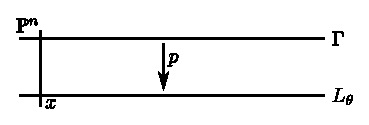
\includegraphics{figures/chap1-fig1.eps}
\end{figure}

Here $A^{+}$ is the point of $s^{+}$ over $\gamma^{+}$, etc., and the
arrows indicate the direction of the $\mathbb{C}^{*}$-flow as $t\to
0$. As the figure indicates $A^{+}$ is the saddle-point over
$\gamma^{+}$ so that $s^{+}$ must coincide with $L^{+}$. Similarly
$B^{-}$ is the saddle-point over $\gamma^{-}$ so that $s^{-}$
coincides with $L^{-}$. Since $s^{+}$ and $s^{-}$ are disjoint it
follows that $L^{+}(x)$ and $L^{-}(x)$ do not coincide. 

Conversely\pageoriginale if $L^{+}(x)\neq L^{-}(x)$ then we get a
diagram as above and we have to deduce that $\mathbb{P}(F)$ is trivial
over $\gamma$. For this consider the closure of a generic
$\mathbb{C}^{*}$-orbit in $\mathbb{P}(F)|_{\gamma}$. From the direction
of the arrows in the diagram we see that this gives a section $\delta$
passing through $A^{-}$ and $B^{+}$. Moreover from \eqref{chap1-eq3.5}
it follows that the intersection numbers $\delta.s^{+}$ and
$\delta.s^{-}$ are both equal to $2p$. This implies that $s^{+}$ and
$s^{-}$ are homologous and from this it follows that
$\mathbb{P}(F)|_{\gamma}$ is indeed a product (for a
$\mathbb{P}_{1}$-bundle over $\mathbb{P}_{1}$ which is not a product,
any two non-intersecting sections have opposite self-intersection
number).

Note that the real structure on $F$ interchanges $L^{+}$ and $L^{-}$
and has to preserve the set of jumping lines. Moreover since $F$ has
no real jumping lines, Proposition \ref{chap1-prop3.5} implies that
$L^{+}$ and $L^{-}$ never coincide at points $x$ for which the line
$\gamma$ (closure of $\mathbb{C}^{*}x$) is real. 

The line bundles $L^{+}$ and $L^{-}$ are in fact {\em algebraic}. This
can be proved by noting that, on
$\mathbb{P}_{3}-(\mathbb{P}^{+}_{1}\cup\mathbb{P}^{-}_{1})$, they
descend to the quotient which is the quadric surface. Since algebraic
line-bundles correspond to algebraic divisor classes and since
divisors on $\mathbb{P}_{3}-\mathbb{P}_{1}$ extend uniquely to
$\mathbb{P}_{3}$ it follows that $L^{+}$ and $L^{-}$ both extend to
line-bundles on $\mathbb{P}_{3}$. Since (ignoring the $\mathbb{C}^{*}$-action) 
$L^+$ restricts to $H^{-k}$ on $\mathbb{P}^{-k}$ on $\mathbb{P}^+_1$ it follows that
$L^+$(and similarly $L^-$) extend to $H^{-k}$ on $\mathbb{P}_3$. 
Moreover, since $\mathbb{P}^{-}_{1}$
has codimension 2, the homomorphism $L^{+}\to F$ extends to a
homomorphism $H^{-k}\to F$. In other words $F(k)=F\otimes H^{k}$ has 
section $\sigma^{+}$ vanishing on $\mathbb{P}^{-}_{1}$, and similarly
a section $\sigma^{-}$ vanishing on $\mathbb{P}^{+}_{1}$. Thus, in the
general correspondence between rank 2 bundles on $\mathbb{P}_{3}$ and
(suitable) algebraic curves, $F$ corresponds to a line with a certain
multiple structure (i.e.\@ a sheaf with nilpotent elements). 

To describe this situation in more detail, it will be necessary to
consider the way in which $\mathbb{C}^{*}$ acts on all this
data. First we\pageoriginale note that the action of $C^{*}$ on
$\mathbb{P}_{3}$ comes from the representation
$$
\lambda\to
\begin{pmatrix}
\lambda^{\sfrac{1}{2}} & & & \\
& \lambda^{\sfrac{1}{2}} & & \\
& & \lambda^{-\sfrac{1}{2}} &\\
&&& \lambda^{-\sfrac{1}{2}}
\end{pmatrix}
$$
on $\mathbb{C}^{4}$. The square-roots indicate that this is really a
representation of the double cover of $\mathbb{C}^{*}$: in fact
$SO(5)\to SO(4)$ is the spin-representation. Let us now denote by
$\mathscr{H}$ the Hopf bundle, regarded as an equivariant bundle for
this action of $\mathbb{C}^{*}$. Then restricting to
$\mathbb{P}^{+}_{1}$ and $\mathbb{P}^{-}_{1}$ we have
\begin{equation}
\mathscr{H}|_{\mathbb{P}^{+}_{1}}\cong H\otimes L^{\sfrac{1}{2}}\quad
\mathscr{H}|_{\mathbb{P}_{1}^{-}}\cong H\otimes
L^{-\sfrac{1}{2}}.\label{chap1-eq3.6} 
\end{equation}
Moreover, the line-bundles $L^{+}$ and $\mathscr{H}^{-k}$ being
isomorphic on $\mathbb{P}_{3}-\mathbb{P}^{-}_{1}$ have
$\mathbb{C}^{*}$-actions which can differ only by a character of
$\mathbb{C}^{*}$ (since all holomorphic functions on
$\mathbb{P}_{3}-\mathbb{P}^{-}_{1}$ are constant). From
\eqref{chap1-eq3.6} we can then deduce that, as equivariant bundles,
\begin{equation}
L^{+}\cong \mathscr{H}^{-k}\otimes L^{p+k/2},\quad L^{-}\cong
\mathscr{H}^{-k}\otimes L^{-p-k/2}\label{chap1-eq3.7}
\end{equation}
Hence the homomorphism $L^{+}\to F$, tensored by $\mathscr{H}^{k}$,
gives a homomorphism $L^{p+k/2}\to F(k)$, showing that the section
$\sigma^{+}$ of $F(k)$ which vanishes on $\mathbb{P}^{-}_{1}$ is of
weight $p+k/2$, i.e.
\begin{equation}
\lambda(\sigma^{+})=\lambda^{p+k/2}\sigma^{+},\quad
\lambda\in\mathbb{C}^{*}\label{chap1-eq3.8} 
\end{equation}

To examine the behaviour of $\sigma^{+}$ near $\mathbb{P}^{-}_{1}$ we
shall use the decomposition \eqref{chap1-eq3.3} which, after twisting
by $\mathscr{H}^{k}$, becomes (using \eqref{chap1-eq3.6}), 
\begin{equation}
F(k)|_{\mathbb{P}^{-}_{1}}\cong L^{-p-k/2}\oplus H^{2k}\otimes
L^{p-k/2}\label{chap1-eq3.9} 
\end{equation}\pageoriginale
Also the canonical bundle $N^{*}$ of $\mathbb{P}^{-}_{1}$ is
$$
N^{*}=H^{-1}\otimes L\otimes\mathbb{C}^{2}
$$
Hence terms of weight $p+k/2$ in the normal Taylor series of
$\sigma^{+}$ can arise in just two ways, namely from
$$
S^{k}(N^{*})\otimes H^{2k}\otimes L^{p-k/2}
$$
and
$$
S^{2p+k}(N^{*})\otimes L^{-p-k/2}.
$$
This shows that, locally, $\sigma^{+}$ is given by a pair of functions
$(f,g)$ where
\begin{equation}
\deg g=k,\quad \deg f=2p+k.\label{chap1-eq3.10}
\end{equation}
This implies that $\mathbb{P}^{-}_{1}$ is a zero of multiplicity
$k(2p+k)$ which proves that
$$
c_{2}(F(k))=2pk+k^{2}
$$
so that
$$
c_{2}(F)=2pk
$$
as we have already proved by other methods.

Since \eqref{chap1-eq3.9} extends as an exact sequence (rather than as
a direct sum) to $\mathbb{P}_{3}-\mathbb{P}^{+}_{1}$, the function $g$
in \eqref{chap1-eq3.10} is globally defined (as a section of $H^{k}$),
but $f$ is only defined locally.
\end{proof}

\section{The mini-twistor picture}\label{chap1-sec4}

In the preceding section, I described the structure of bundles on the
twistor space $\mathbb{P}_{3}$ corresponding to $S^{1}$-invariant
instantons.\pageoriginale Because these bundles are acted on by
$\mathbb{C}^{*}$ it is possible to descend these bundles to the
quotient space
\begin{equation}
Q=\frac{\mathbb{P}_{3}-(\mathbb{P}^{+}_{1}\cup
  \mathbb{P}^{-}_{1})}{\mathbb{C}^{*}}\label{chap1-eq4.1} 
\end{equation}
Since any point $x$ in $\mathbb{P}_{3}-(\mathbb{P}^{+}_{1}\cup
\mathbb{P}^{-}_{1})$ lies on a unique transversal to
$\mathbb{P}^{+}_{1}$ and $\mathbb{P}^{-}_{1}$ this transversal is the
closure of the $\mathbb{C}^{*}$-orbit through $x$. This shows that
\begin{equation}
Q\cong \mathbb{P}\times \mathbb{P}^{-}_{1}\label{chap1-eq4.2}
\end{equation}
so that $Q$ is (abstractly) a quadric surface. Moreover the real
structure on $P_{3}$ induces a real structure on $Q$ which
interchanges the two factors, and the real points form the
``anti-diagonal'' $Q^{\sigma}$ consisting of pairs
$(y,\sigma(y))$. Thus the bundle $F$ on $\mathbb{P}_{3}$ descends to a
bundle, say $\mathscr{F}$, on $Q$, and $\mathscr{F}$ also has a real
structure. 

Since $\mathbb{P}^{+}_{1}$ and $\mathbb{P}^{-}_{1}$ have co-dimension
2 in $\mathbb{P}_{3}$ two bundles on $\mathbb{P}_{3}$ which are
isomorphic on $\mathbb{P}_{3}-(\mathbb{P}^{+}_{1}\cup
\mathbb{P}^{-}_{1})$ are automatically isomorphic on
$\mathbb{P}_{3}$. Thus $\mathscr{F}$ uniquely determines $F$, so that
no information has been lost on descending to $Q$. We proceed now to
reinterpret the results on \S\ \ref{chap1-sec3} in terms of bundles on
$Q$. 

The sub-line-bundle $L^{+}$ of $F$ descends to a sub-line-bundle
$\mathscr{L}^{+}$ of $\mathscr{F}$. If we denote by $H_{+}$ and
$H_{-}$ the Hopf bundles on $P^{+}$ and $\mathbb{P}^{-}_{1}$ pulled
back to $Q$ by the factorization \eqref{chap1-eq4.2}, then
$\mathscr{L}^{+}$ must be of the form $H^{\alpha}_{+}\otimes
H^{\beta}_{-}$ for some integers $\alpha$, $\beta$. 
To find these we use \eqref{chap1-eq3.7} which can also be rewritten
\setcounter{equation}{1}
\begin{equation}
L^{+}\cong \pi^{*}_{+}(H^{-k}\otimes L^{p})\cong
\pi^{*}_{1}(H^{-k}\otimes L^{+k})\label{addchap1-eq4.2} 
\end{equation}
where\pageoriginale $\pi_{\pm}:\mathbb{P}_{3}-\mathbb{P}^{\mp}_{1}\to
\mathbb{P}^{\pm}_{1}$ are the natural linear projections. Restricting
$L^{+}$ to the plane $\pi^{-1}_{+}(y)$ for $y\in \mathbb{P}^{+}_{1}$
and using the first isomorphism in \eqref{addchap1-eq4.2} then shows that
\begin{equation}
\mathscr{L}^{+}|_{y\times \mathbb{P}_{1}^{-}}\cong
H^{p}_{-}\label{chap1-eq4.3} 
\end{equation}
so that $\beta=p$. Similarly the second isomorphism in
\eqref{chap1-eq4.2} shows that $\alpha=-(p+k)$. Hence
\begin{equation}
\mathscr{L}^{+}\cong H^{-p-k}_{+}\oplus H^{p}_{-};\label{chap1-eq4.4}
\end{equation}
similarly, we find
\begin{equation}
\mathscr{L}^{-}\cong H^{p}_{+}\oplus H^{-p-k}_{-}\label{chap1-eq4.5}
\end{equation}

Thus the bundle $\mathscr{F}$ on $Q$ has two different splittings:
\begin{align}
& 0\to \mathscr{L}^{+}\to \mathscr{F}\to (\mathscr{L}^{+})^{*}\to
  0\notag\\
& 0\to \mathscr{L}^{-}\to \mathscr{F}\to (\mathscr{L}^{-})^{*}\to
  0\label{chap1-eq4.6} 
\end{align}
where $\mathscr{L}^{+}$ and $\mathscr{L}^{-}$ are given by
\eqref{chap1-eq4.4} and \eqref{chap1-eq4.5}. Moreover these splittings
are interchanged by the linear structure.

These two splittings coincide where the composite homomorphism
$$
\mathscr{L}^{+}\to \mathscr{F}\to (\mathscr{L}^{-})^{*}
$$
is zero. This is given by the vanishing of a section $s$ of the line
bundle
\begin{equation}
(\mathscr{L}^{+}\otimes \mathscr{L}^{-})^{*}\cong (H_{+}\otimes
  H_{-})^{k}\label{chap1-eq4.7} 
\end{equation}
The\pageoriginale zero set of $s$ is therefore a curve $S$ on $Q$ of
bidegree $(k,k)$. The curve $S$ is real and the line-bundles
$\mathscr{L}^{+}$ and $\mathscr{L}^{-}$. coincide over $S$ so that
\begin{equation}
H^{2p+k}_{+}|_{s}\cong H^{2p+k|s}_{-}\label{chap1-eq4.8}
\end{equation}
More geometrically this means that, if $D_{+}$, $D_{-}$ are the
divisors cut out on $S$ by the two systems of generators of $Q$, then 
\begin{equation}
(2p+k)(D_{1}-D_{2})\approx 0\label{chap1-eq4.9}
\end{equation}
where $\approx$ denotes linear equivalence on $S$.

Following Hitchin \cite{chap1-key7}, we shall call $S$ the {\em
  spectral curve} of the hyperbolic monopole. Just as in
\cite{chap1-key7}, $S$ determines the monopole uniquely. In fact
consider the exact sequence of sheaves on $Q$
$$
0\to\mathscr{O}(-2p-2k,2p)\to \mathscr{O}(-2p-k,2p+k)\to
\mathscr{O}_{s}\to 0
$$
where $\mathscr{O}(\alpha,\beta)$ denotes sections of
$H^{\alpha}_{+}\otimes H^{\beta}_{-}$ and we have used
\eqref{chap1-eq4.8}. Taking
$$
\delta(1)\in H^{1}(Q,\mathscr{O}(-2p-2k,2p))=H^{1}(Q,(\mathscr{L}^{+})^{2})
$$
where $\delta$ is the coboundary in the cohomology exact sequence we
get the element which defines the first extension in \eqref{chap1-eq4.6}
and so recover $\mathscr{F}$. 

Finally, we note that $\mathscr{F}$, restricted to a generator of $Q$
of either system, has constant type $H^{p}\oplus H^{-p}$. This follows
at once by using the splittings \eqref{chap1-eq4.6} together with the
isomorphisms \eqref{chap1-eq4.4} and \eqref{chap1-eq4.5}. Thus, for
restricted to a $\mathbb{P}_{-}$ generator, we use the first extension
of \eqref{chap1-eq4.6} and get an extension 
$$
0\to H^{p}_{-}\to \mathscr{F}|_{\mathbb{P}_{-}}\to H^{-p}_{-}\to 0
$$\pageoriginale
which splits since $p>0$.

The fact that the restriction of $\mathscr{F}$ to the generators is
not generically trivial means that the extension classes in
\eqref{chap1-eq4.6} are very special. This is borne out by a parameter
count which shows that the space of all extensions of the form
\eqref{chap1-eq4.6} is much larger than the moduli space of
monopoles. Moreover the fact that decomposition is of constant type,
i.e.\@ that there are no special generators, guarantees that the
bundle $\mathscr{F}$ when lifted back to
$\mathbb{P}_{3}-\mathbb{P}^{+}_{1}\cup \mathbb{P}^{-}_{1}$) {\em
  extends} to $\mathbb{P}_{3}$. Special generators would mean that
$\mathscr{F}$ would only extend as a torsion-free sheaf, having a
finite number of special points on $\mathbb{P}^{+}_{1}$,
$\mathbb{P}^{-}_{1}$ where it was not locally free.

When $k=1$, the spectral curve $S$, being of bidegree $(1,1)$ is a
conic section and so corresponds to a point $0$ in $H^{3}$. All
geodesics through this point are then ``spectral lines''. Moreover
since the monopole is uniquely determined by $S$ it follows that it is
rotationally symmetric about $0$. We may therefore refer to $0$ as the
{\em centre} of the monopole, and the situation is quite analogous to
that for Euclidean 3-space.

\section{The limiting process}\label{chap1-sec5}

Comparison of the results of \S\ \ref{chap1-sec4} with those of
Hitchin \cite{chap1-key7} show that the mini-twistor pictures of
hyperbolic and Euclidean monopoles are quite similar. The holomorphic
bundle on the mini-twistor space has in each case two canonical
splittings (conjugates of each other) and a spectral curve where they
coincide, which determines the monopole. The main difference is that
in the Euclidean case the splittings are defined by asymptotic
behaviour, where as in the hyperbolic case we have a compactification
which incorporates infinity. 

To\pageoriginale pursue the comparison further, let us, following
Hitchin, consider the case of $U(1)$-monopoles on hyperbolic
space. For these, the connection is flat and the Higgs field is the
constant i. This corresponds to the trivial line bundle on $S^{4}$ (or
on its twistor space $\mathbb{P}_{3}$) with the standard
$S^{1}$-action. As we saw in \S\ \ref{chap1-sec4}, this descends from
$\mathbb{P}_{3}$ to the quadric $Q$ to give the line bundle
$H^{-1}_{+}\otimes H_{-}$. This is therefore the analogue of Hitchin's
line bundle $L$ on $T\mathbb{P}_{1}$ (the tangent bundle of
$\mathbb{P}_{1}$). Comparing \eqref{chap1-eq4.4} and
\eqref{chap1-eq4.6} with theorem (6.3) of \cite{chap1-key7} then shows
that they are precisely of the same form.

So far, we have only considered the standard hyperbolic space with
curvature $-1$. We now want to vary the curvature and then consider
the limiting situation when the curvature tends to zero, giving flat
Euclidean space. If, for some positive constant $R$, we rewrite
\eqref{chap1-eq2.3} as 
\begin{equation}
ds^{2}=\dfrac{r^{2}}{R^{2}}\left\{R^{2}\left\{\dfrac{dx^{2}+dy^{2}+dr^{2}}{r^{2}}\right\}+R^{2}d\theta^{2}\right\}\label{chap1-eq5.1} 
\end{equation}
this replaces \eqref{chap1-eq2.4} by the conformal equivalence
\begin{equation}
\mathbb{R}^{4}-\mathbb{R}^{2}\sim H^{3}(R)\times S^{1}(R)\label{chap1-eq5.2}
\end{equation}
where $S^{1}(R)$ is the circle of radius $R$ and $H^{3}(R)$ is
hyperbolic space of curvature $-R^{-}$. An $S^{1}$-invariant instanton
of weight $p$ on $R^{4}$ thus defines a monopole on $H^{3}(R)$ in
which, because of the scale change on the circle, the norm of the
Higgs field tends to $R^{-1}p$ at infinity. In particular, taking
$R=p$ we see that monopoles on $H^{3}$ with $|\phi|\to p$ at $\infty$
are equivalent, by this rescaling, to monopoles on $H^{3}(p^{-1})$
with $|\phi|\to 1$ at $\infty$. Note that in Euclidean space, because
there is no absolute scale, we can always renormalize the Higgs field
to have $|\phi|\to 1$.

The\pageoriginale idea now is that, as $p\to \infty$, monopoles on the
sequence of spaces $H^{3}(p^{-1})$ should in some appropriate sense
converge to monopoles on Euclidean space, the Higgs field having
throughout been normalized so that $|\phi|\to 1$ at $\infty$. More
precisely, let us represent $H^{3}(R)$ as the ball of radius $R$ in
Euclidean 3-space. It is easy to show that, as $R\to \infty$, the
hyperbolic metrics of these balls converge, on any compact set, to the
Euclidean metric. It now makes sense to ask that a sequence of
hyperbolic monopoles defined on each $B(p)$, should converge to a
Euclidean monopole as $p\to \infty$. If the sequence converges
smoothly, it is clear that the limit will indeed be a Euclidean
monopole.

If we reinterpret hyperbolic monopoles as $S^{1}$-invariant
instantons, this limiting procedure amounts to considering (backward)
rotations in the $(x_{3},x_{4})$-plane having centres at $(0,0,p,0)$
and using as $S^{1}$-parameter the arc length of the orbit through the
origin (divided by $2\pi$). In terms of the generating vector fields,
these are normalized to have length one at the origin. As $p\to
\infty$, these vector fields converge, on any compact set, to the
generator of translation in the $x_{4}$-direction.
\begin{figure}[H]
\centering
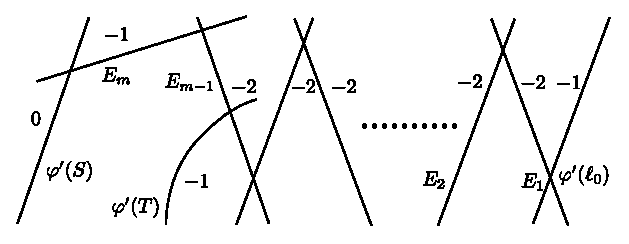
\includegraphics{figures/chap1-fig2.eps}
\end{figure}
These vector fields then induce holomorphic vector fields $\xi_{p}$ on
$\mathbb{P}_{3}$, generating $C^{*}$-actions and converging as $p\to
\infty$ to a $\mathbb{C}$-action.

For the standard $S^{1}$-action considered in \S\ \ref{chap1-sec4} the
$\mathbb{C}^{*}$-fibration over $Q$ defined by \eqref{chap1-eq4.1} is
easily seen (by calculations similar to those in \S\ \ref{chap1-sec4})
to define the line-bundle $H_{+}\otimes H^{-1}_{-}$. Reversing
the\pageoriginale orientation of $S^{1}$ leads to the inverse
$H^{-1}_{+}\otimes H$ while rescaling replaces the bundle by its
powers. Hence the vector field $\xi_{p}$ induces the standard action
of $\mathbb{C}^{*}=\mathbb{C}/2\pi\mathbb{Z}$ on
$L_{p}=H^{-p}_{+}\otimes H^{p}$ over the quadric $Q_{p}$: the
principal bundle of $L_{p}$ can be identified with the quotient of
$\mathbb{P}_{3}-(\mathbb{P}^{+}_{1}(\mathbb{P})\cup
\mathbb{P}^{-}_{1}(p))$ by $Z_{p}$, ($P_{1}(p)$ denoting the zeros of
$\xi_{p}$). 

If we introduce
\begin{equation}
\widetilde{Q}_{p}=Q_{p}-Q_{p}^{\sigma}\label{chap1-eq5.3}
\end{equation}
the complement of the real points of $Q_{p}$, then $L_{p}$ is
topologically trivial on $\widetilde{Q}_{p}$ and arises by
exponentiation from an element of $H^{1}(Q_{p},\mathscr{O})$. This
element can be viewed geometrically as the -bundle given by the action
$t\to \exp 2\pi t\xi_{p}$ on the universal covering space of
$\widetilde{P}_{p}$, where
$\widetilde{P}_{p}=\pi^{-1}(\mathbb{R}^{2}-\mathbb{R}^{2}_{p})$,
$R^{2}_{p}$ is the axis of the $p$th rotation and
$\pi:\mathbb{P}_{3}\to S^{4}$ is the twistor fibration. Note that at
this stage $p$ could be any positive {\em real} number, the
integrality is only needed if we deal with the whole of $Q_{p}$ rather
than the open set $\widetilde{Q}_{p}$.

As $p\to\infty$ the quadrics $Q_{p}$ tend to the quadric cone
$T\mathbb{P}_{1}$, and this degeneration is best viewed by realizing
the $Q_{p}$ as all embeded in a fixed projective 3-space. I shall now
describe such a realization.

Recall first that $TP_{1}$ parametrizes oriented straight lines in the
Euclidean 3-space $V=\mathbb{R}^{3}$, and that points of
$\mathbb{R}^{3}$ correspond to real sections of $T\mathbb{P}_{1}$. One
way to derive this correspondence is to introduce the affine dual $V'$
of $V$, i.e.\@ the space parametrizing affine planes in $V$. If we
introduce the projective space $\mathbb{P}$ compactifying $V$ and its
projective dual $\mathbb{P}'$ then $V'\subset \mathbb{P}$ is the
complement of one point. If $x$, $y$, $z$ are coordinates for $V$, $t$
a fourth homogeneous coordinate and 
\begin{equation}
\xi x+\eta y+\zeta z+\tau t=0\label{chap1-eq5.4}
\end{equation}
the\pageoriginale equation of a projective plance, then
$(\xi,\eta,\zeta,\tau)$ are homogeneous coordinates for $\mathbb{P}'$
and $V'$ is the complement of the point $(0,0,0,1)$. Now an affine
line $L\subset V$ has a dual line $L'\subset V'$ and, if we
complexity, the line $L'_{\mathbb{C}}$ meets the complex quadric cone
\begin{equation}
\xi^{2}+\eta^{2}+\zeta^{2}=0\label{chap1-eq5.5}
\end{equation}
in a pair of complex conjugate points. An orientation of $L$ gives a
preferred choice of one of these points and in this way affine lines
$L\subset V$ are parametrized by points of the cone
\eqref{chap1-eq5.5}, excluding the vertex $(0,0,0,1)$. Note that
\eqref{chap1-eq5.5} is the dual of the (purely imaginary) conic at
$\infty$ in $\mathbb{P}_{\mathbb{C}}$ given by
\begin{equation}
x^{2}+y^{2}+z^{2}=0,\quad t=0\label{chap1-eq5.6}
\end{equation}
which arises from the Euclidean metric structure of $V$.

Now consider the hyperbolic space $H^{3}(R)$ and identify it as before
with the ball $B(R)\subset V$. A hyperbolic plane in $B(R)$ is
determined by its ``circle at $\infty$'', i.e. on the boundary of
$B(R)$. This is cut out by a plane in $V$, so that the affine dual
$B(R)'$ of $B(R)$ can be identified with the subspace of $V'$
representing planes in $V$ whose distance to the origin is less than
$R$. Thus $B(R)$ is given by the inequality
\begin{equation}
\xi^{2}+\eta^{2}+\zeta^{2}-R^{-2}\tau^{2}>0.\label{chap1-eq5.7}
\end{equation}
A geodesic in $B(R)$ is therefore represented by a line $L'$ inside
the region \eqref{chap1-eq5.7}. The analogue of \eqref{chap1-eq5.5} is
the complex quadric in $\mathbb{P}'_{\mathbb{C}}$ given by the
equation
\begin{equation}
\xi^{2}+\eta^{2}+\zeta^{2}-R^{-2}\tau^{2}=0\label{chap1-eq5.8}
\end{equation}
which\pageoriginale is the dual of the equation
\begin{equation}
x^{2}+y^{2}+z^{2}-R^{2}t^{2}=0\label{chap1-eq5.9}
\end{equation}
giving the complexification of the boundary of $B(R)$. The
complexification $L'_{\mathbb{C}}$ meets \eqref{chap1-eq5.8} in a pair
of conjugate points and, as before, an orientation of the geodesic
gives a preferred choice. Note that as $L'$ lies inside the region
\eqref{chap1-eq5.7} it does not meet the quadric \eqref{chap1-eq5.8},
so that our points are never real. In this way, oriented geodesics
$B(R)$ are naturally parametrized by the non-real points
$\widetilde{Q}(R)$ of the quadric $Q(R)$ given by \eqref{chap1-eq5.8}.

As $R\to \infty$, the quadric $Q(R)$ tends to the quadric cone given
by \eqref{chap1-eq5.5} and it is not hard to see that parametrization
of (oriented) geodesics is continuous. Thus, if $\alpha_{R}$ is an
oriented geodesic in $B(R)$ which converges (on compact sets) to a
straight line as $R\to \infty$, then the corresponding points on
$Q(R)$ converge to the required point on the cone.

I shall now describe the family of line-bundles $L_{R}$ on $Q(R)$ and
show that they converge to Hitchin's line bundle $L$ on
$Q(\sfrac{1}{2})=TP_{1}$. 

Let $U$ be the open set $\eta\neq i\xi$ and $V$ the open set $\eta\neq
-i\xi$. Their union covers $\widetilde{Q}(R)$ because the excluded
line $\xi=\eta=0$ intersects $Q(R)$ in the {\em real} points
$(0,0,1,\pm R)$. The transition function
$$
g_{UV}=\dfrac{\zeta+R^{-1}\tau}{\zeta-R^{-1}\tau}
$$
is holomorphic and non-zero on $U\cap V\cap Q_{R}$ and it defines a
line-bundle on $Q_{R}$. This is, in fact, the restriction of the line
bundle $H^{-1}_{+}\otimes H_{-}$ on $Q_{R}$.

Consider\pageoriginale now the line bundle $L_{R}$ on
$\widetilde{Q}(R)$ defined by the transition function
$(g_{UV})^{R}$. As $R\to \infty$, this converges to the limit
\begin{equation}
g^{\infty}_{UV}=\exp (2\tau/\zeta)\label{chap1-eq5.10}
\end{equation}
defining a line-bundle $L_{\infty}$ on
$\widetilde{Q}(\infty)=T\mathbb{P}_{1}$. It remains to check that
$L_{\infty}$ coincides with Hitchin's line-bundle $L$. Now, in our
coordinates, a point $(a,b,c)\in \mathbb{R}^{3}$ is represented by the
plane 
\begin{equation}
a\xi+b\eta+c\zeta=\tau.\label{chap1-eq5.11}
\end{equation}
If we now parametrize $\mathbb{P}_{1}$, defined by the homogeneous
equation \eqref{chap1-eq5.4}, by
$$
\frac{\xi}{\zeta}=\dfrac{\rho-\rho^{-1}}{2},\quad \frac{\eta}{\zeta}=\dfrac{\rho+\rho^{-1}}{2i}
$$
then \eqref{chap1-eq5.11} becomes
\begin{equation}
\tau/\zeta=-\sfrac{1}{2}\left\{(a+ib)\rho^{-1}-2c-(a-ib)\rho\right\}\label{chap1-eq5.12} 
\end{equation}
Comparing this with \eqref{chap1-eq3.2} of \cite{chap1-key1} shows
that our coordinates are related to Hitchin's by
$$
\rho\to \zeta\quad \tau/\zeta\to -\eta/2.
$$
Thus our formula \eqref{chap1-eq5.10} coincides with Hitchin's formula
\eqref{chap1-eq5.4} in \cite{chap1-key7}, showing that out
$L_{\infty}$ is his $L$.

\section{The moduli space}\label{chap1-sec6}

In \cite{chap1-key2} I showed, using a recent result of Donaldson
\cite{chap1-key4}, that the moduli space of (based) monopoles of
charge $k$ on the hyperbolic space $H^{3}$ can naturally be identified
with the space\pageoriginale of based holomorphic maps
$\mathbb{P}_{1}\to \mathbb{P}_{1}$ of degree $k$, i.e.\@ with the
space of rational functions
$$
f(z)=\dfrac{a_{1}z^{k-1}+a_{2}z^{k-2}+\cdots+a_{k}}{z^{k}+b_{1}z^{k-1}+\cdots+b_{k}} 
$$
where the numerator and denominator have no common factor. In
\cite{chap1-key2}, this was deduced as a special case of a more
general result for instantons. I shall now give a more direct and
elementary treatment for the case of monopoles alone. Again this rests
on \cite{chap1-key4} and the proof is not essentially different from
that in \cite{chap1-key2}, but the presentation is simpler and gives
more insight into the way the moduli space arises.

An instanton on $\mathbb{R}^{4}$ (or $S^{4}$) defines a holomorphic
bundle on the twistor space $\mathbb{P}_{3}$ with a real structure
(and satisfying further a non-degeneracy condition). If we pick a
plane $\mathbb{P}_{2}$ in $\mathbb{P}_{3}$ and restrict the bundle, we
get a holomorphic bundle on $\mathbb{P}_{2}$ trivial on the unique
real line in $\mathbb{P}_{2}$. Donaldson's result in \cite{chap1-key4}
asserts that this process identifies the moduli space of based
instantons on $S^{4}$ with that of holomorphic bundles on
$\mathbb{P}_{2}$ trivialized on $\mathbb{P}_{1}$. Here a base bundle
means a bundle with a preferred choice of trivialization over some
base point. The important point in this result of Donaldson is that
the bundles on $\mathbb{P}_{2}$ are purely holomorphic - there is no
real or unitary restriction, and $SU(2)$ gets replaced by
$SL(2,\mathbb{C})$. 

For an $S^{1}$-invariant instanton we pick our $\mathbb{P}_{2}$ to
contain the fixed line $\mathbb{P}^{+}_{1}$ and we take as base point
its intersection $A$ with $\mathbb{P}^{-}_{1}$. Then $\mathbb{P}_{2}$
is also $S^{1}$-invariant and the naturality of Donaldson's theorem
implies that the moduli space of based monopoles on $H^{3}$ can be
identified with the moduli space of $S^{1}$-invariant based bundles on
$\mathbb{P}_{2}$. Note that the $S^{1}$-action does not preserve
the\pageoriginale trivilization over the base point $A$. In fact, the
representation of $S^{1}$ on the fibre over $A$ is determined by the
Higgs field.

The action of $S^{1}$ complexifies to an action of $\mathbb{C}^{*}$
and both the bundle on $\mathbb{P}_{2}$ and the
$\mathbb{C}^{*}$-action are necessarily {\em algebraic}. The
classification of such objects is a fairly elementary matter as we
shall now see. As a first step, let us prove:

\begin{lemma}\label{chap1-lem6.1}
Let $E$ be an algebraic vector bundle of rank $n$ over
$\mathbb{C}^{2}$ with an action of $\mathbb{C}^{*}$ covering the
scalar action on $\mathbb{C}^{2}$. Then $E$ is
$\mathbb{C}^{*}$-isomorphic to the product $\mathbb{C}^{2}\times
E_{O}$. 
\end{lemma}

\begin{proof}
$\mathbb{C}^{*}$-bundles on $\mathbb{C}^{2}-0$ are equivalent to
  bundles on the quotient space $\mathbb{P}_{1}$. By Grothendieck's
  theorem, every vector bundle on $\mathbb{P}_{1}$ is a direct sum of
  powers of the Hopf bundle. Hence on $\mathbb{C}^{2}-0$ every
  $\mathbb{C}^{*}$-vector bundle is isomorphic to a product bundle of
  the form $(\mathbb{C}^{2}-0)\times V$, where $V$ is a representation
  of $\mathbb{C}^{*}$ (and so a sum of one-dimensional
  representations). Thus our bundle $E$ and the product
  $\mathbb{C}^{2}\times V$ are $\mathbb{C}^{*}$-isomorphic on
  $\mathbb{C}^{2}-0$. The isomorphism then necessarily extends to
  $\mathbb{C}^{2}$ and induces in particular an isomorphism of
  representations of $\mathbb{C}^{*}$ between $E_{O}$ and $V$.

We shall be interested in the case $n=2$ and representations with
weights $(p,-p)$ for $p>0$. The proof of Lemma \ref{chap1-lem6.1} also
shows that the $\mathbb{C}^{*}$-automorphisms of
$E=\mathbb{C}^{2}\times E_{O}$ are all of the form
\setcounter{equation}{1}
\begin{equation}
(z_{1},z_{2};u,v)\to (z_{1},z_{2};au+c(z_{1},z_{2})v,bv)\label{chap1-eq6.2}
\end{equation}
where $a$, $b$ are non-zero constants and $c(z_{1},z_{2})$ is a
homogeneous polynomial of degree $2p$. Here $\lambda\in
\mathbb{C}^{*}$ is taken to act on $E_{O}$ by
$$
(u,v)\to \left(\lambda^{p}_{u}, \lambda^{-p}_{v}\right).
$$

By lifting a bundle from $\mathbb{C}^{1}$ to $\mathbb{C}^{2}$ and
applying \ref{chap1-lem6.1} and \eqref{chap1-eq6.2}, we deduce:
\end{proof}

\setcounter{theorem}{2}
\begin{corollary}\label{chap1-coro6.3}
Lemma\pageoriginale \ref{chap1-lem6.1} holds with $\mathbb{C}^{1}$ instead of
$\mathbb{C}^{2}$ and automorphisms for $n=2$ and weights $(p,-p)$ are
given by
$$
(z;u,v)\to (z;~au+cz^{2p},bv)\quad\text{with}\quad ab\neq 0
$$
\end{corollary}

\begin{remark*}
The analogue of \ref{chap1-lem6.1} holds for bundles over
$\mathbb{C}^{m}$ for any $m$, but we only need the cases $m=1,2$ and
the proof for $m\geq 3$ is slightly more complicated.
\end{remark*}

Suppose next that $E$ is a $\mathbb{C}^{*}$-vector bundle over
$\mathbb{P}_{1}=\mathbb{C}\cup \infty$. Then we have representations
$E_{O}$ and $E_{\infty}$ which by \eqref{chap1-coro6.3}
determine $E$ restricted to the two open sets $\mathbb{P}_{1}-\infty$
and $\mathbb{P}_{1}-0$. Over the intersection $\mathbb{C}^{*}$-bundles
are equivalent to bundles over a point, so that the data needed to
construct $E$ from $E_{O}$ and $E_{\infty}$ is just a vector space
isomorphism $T:E_{O}\to E_{\infty}$ (not necessarily commuting with
the action of $\mathbb{C}^{*}$). For example, $T$ could be fixed by
looking at the fibre over the point $z=1$. Changing the identification
$$
E|_{\mathbb{P}_{1}-\infty}\cong (\mathbb{P}_{1}-\infty)\times E_{O}
$$
by an automorphism of $(\mathbb{P}_{1}-\infty)\times E_{O}$ alters $T$
to $TS$. In the case we want, when $n=2$ and the weights of $E_{O}$
are $(p,-p)$, Corollary \eqref{chap1-coro6.3} shows that $S$ is
(relative to the standard basis) given by {\em a triangular
  matrix}. The coset space of the triangular matrix group in
$GL(2,\mathbb{C})$ is just the projective line. More invariantly, let
$$
\mathbb{P}(T):\mathbb{P}(E_{O})\to \mathbb{P}(E_{\infty})
$$
be the projective isomorphism induced by $T$, and let $p_{O}\in
P(E_{O})$ correspond to the positive weight vector. This is the point
fixed by the automorphism $S$. Hence the left cosets of $S$ are
determined by the point
\setcounter{equation}{3}
\begin{equation}
\mathbb{P}'(T)(p_{O})\in \mathbb{P}(E_{\infty}).\label{chap1-eq6.4}
\end{equation}\pageoriginale

Summing up this discussion, we see that we have proved the following:

\setcounter{theorem}{4}
\begin{proposition}\label{chap1-prop6.5}
Let $E$ be a $\mathbb{C}^{*}$-vector bundle of rank $2$ over $P_{1}$
with $E_{O}$ having weights $(p,-p)$, and with a preferred
$\mathbb{C}^{*}$-isomorphism
$$
E|_{\mathbb{P}_{1}-0}\cong (\mathbb{P}_{1}-0)\times E_{\infty}. 
$$
Then $E$ corresponds canonically to a point of
$\mathbb{P}(E_{\infty})$. 
\end{proposition}

\begin{remark*}
The matrix $T:E_{O}\to E_{\infty}$ defined earlier should be viewed as
a kind of ``scattering matrix'' and the point in
$\mathbb{P}(E_{\infty})$ as the ratio of the
``reflection/transmission'' coefficients. I shall have more to say
about this later. 
\end{remark*}

We are now ready to return to the $\mathbb{C}^{*}$-bundle $E$ over
$\mathbb{P}_{2}$ corresponding, by Donaldson, to an $S^{1}$-invariant
instanton and so to a hyperbolic monopole. Recall that
$\mathbb{P}_{2}$ contains a fixed point $A$ {\em and} a fixed line
$\mathbb{P}^{+}_{1}$, and a unique real line, joining $A$ to its
conjugate point $A^{*}$ on $\mathbb{P}^{+}_{1}$
\begin{figure}[H]
\centering
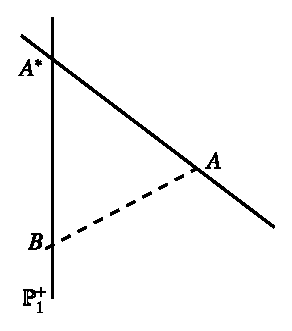
\includegraphics{figures/chap1-fig3.eps}
\end{figure}

The bundle $E$ is trivial on the line $AA^{*}$ and hence on all nearby
lines through $A^{*}$. Applying the action of $\mathbb{C}^{*}$ then
shows that $E$ is trivial on all lines through $A^{*}$ except
$\mathbb{P}^{+}_{1}$. The trivialization of $E$ on $AA^{*}$ then
extends to all these lines. In particular we get a distinguished
$\mathbb{C}^{*}$-isomorphism 
$$
E|\mathbb{P}_{2}-\mathbb{P}^{+}_{1}\cong
(\mathbb{P}_{2}-\mathbb{P}^{+}_{1})\times E_{A}.
$$\pageoriginale

Now apply \eqref{chap1-prop6.5} to the bundle $E$ restricted to a
variable line $BA$ using a third fixed line through $A^{*}$ to define
the unit point (and so identifying $BA$ with the standard
$\mathbb{P}_{1}$). We deduce that $E$ corresponds canonically to a
rational map
\setcounter{equation}{5}
\begin{equation}
f:\mathbb{P}^{+}_{1}\to \mathbb{P}(E_{A}).\label{chap1-eq6.6}
\end{equation}
Actually, our construction only defines $f$ on
$\mathbb{P}^{+}_{1}-A^{*}$ but, because the trivializations emanate
from $A^{*}$ it is easy to see that $f$ extends by continuity to the
whole of $\mathbb{P}^{+}_{1}$. 

If we compare the definition of \eqref{chap1-eq6.6} with proposition
\eqref{chap1-eq3.5} we see that the poles of $f$ occur precisely at
the $k$ points $B$ for which $BA$ is a jumping line of $E$. To be
precise, we parametrize $\mathbb{P}(E_{A})\cong \mathbb{P}(E_{A^{*}})$
so that $\infty$ corresponds to the minimum weight vector, and $0$ to
the maximal weight vector. Note that $f(A^{*})=0$.

This completes the proof that the moduli space of based monopoles of
charge $k$ on $H^{3}$ is the space $M_{k}$ of based rational maps
$\mathbb{P}_{1}\to \mathbb{P}_{1}$ of degree $k$. Note that the moduli
space is independent of the weight $p$, i.e.\@ of the norm of the
Higgs field at $\infty$. This makes it very plausible that, in the
limiting procedure described in \S\ \ref{chap1-sec5} for $p\to
\infty$, the moduli spaces should converge to the corresponding moduli
space for Euclidean monopoles, which has already been proved by
Donaldson \cite{chap1-key5} to coincide with $M_{k}$. Moreover if we
allow non-integral values of $p$ we should get a nice continuous
one-parameter family of moduli spaces.

So far we have defined the rational map $f$ in \eqref{chap1-eq6.6}
purely from the holomorphic point of view. In fact it has quite a
simple interpretation from the monopole point of view. To see this let
us first project from the twistor space $\mathbb{P}_{3}$ back to
$S^{4}$. Then\pageoriginale our plane $\mathbb{P}_{2}$ maps to $S^{4}$
with the line $AA^{*}$ collapsing to the point at $\infty$ and
$\mathbb{C}^{2}=\mathbb{P}_{2}-(AA^{*})$ gets identified with
$\mathbb{R}^{4}$. This identification is compatible with the
$\mathbb{C}^{*}$-action so the fixed line $\mathbb{P}^{+}_{1}$ (with
$A^{*}$ deleted) maps to the $\mathbb{R}^{2}$ axis in $R^{4}$, while
the lines $BA$ (with $A$ deleted) map to the plane orthogonal to this
axis. As before we introduce coordinates $(x,y,r,\theta)$.

The rational map $f$ determined by a monopole is defined at a point
$x_{0}+iy_{0}$ by considering the $\mathbb{C}^{*}$-bundle over the
projective line $\mathbb{P}_{1}(x_{0},y_{0})$ (obtained by
compactifying the plane $x=x_{0}$, $y=y_{0}$) and applying Proposition
\eqref{chap1-prop6.5}. Here the complex coordinate of this
$\mathbb{P}_{1}$ is $w=re^{i\theta}$. The procedure to obtain the
value $f(x_{0}+iy_{0})$ is now as follows.

Over $\mathbb{C}=\mathbb{P}_{1}-\infty$ our bundle can be described as
a product $\mathbb{C}\times \mathbb{C}^{2}$ with coordinates $(w;u,v)$
and $\mathbb{C}^{*}$-action given by 
$$
\lambda(w;u,v)=(\lambda w;\lambda^{p}_{u},\lambda^{-p}_{v}).
$$
There are two distinguished (invariant) sections, namely
\begin{align*}
& s_{+}:u=w^{p},\quad v=0,\\
& s_{-}:u=0,\quad v=w^{-p}.
\end{align*}
Notice that the first is holomorphic on $\mathbb{C}$ while the second
has a pole at $0$. Similarly over $\mathbb{P}_{1}-0$ we have
coordinates $(w';u',v')$ with similar formulae, and distinguished
sections $s'_{+}$, $s'_{-}$ with $s'_{+}$ holomorphic at $\ell$. In
the overlap $\mathbb{P}_{1}-(0\cup \infty)$ we have the ``scattering
matrix'' $T$ expressing $s_{\pm}$ in terms of $s'_{\pm}$:
\begin{align*}
& s_{+}=as'_{+}+bs'_{-}\\[3pt]
& s_{-}=cs'_{+}+ds'_{-}
\end{align*}
with\pageoriginale $a$, $b$, $c$, $d$ constants. The value of
$f(x_{0}+iy_{0})$ is then $a/b$: note that a pole of $f$, i.e. having
$b=0$, corresponds to $\mathbb{P}_{1}$ being a jumping line. 

We shall now translate this into monopole terminology on the
hyperbolic space $H^{3}$, given as the upper half space
\begin{equation}
(x,y,r)~r>0.\label{chap1-eq6.7}
\end{equation}
If we put $\rho=\log r$, so that $\rho+i\theta=\log w$, holomorphic
sections $s$ of $E$ over $\mathbb{P}_{1}$ are defined to be solutions
of the equation
\begin{equation}
\nabla_{\rho^{s}}+i\nabla_{\theta^{s}}=0\label{chap1-eq6.8}
\end{equation}
where $\nabla_{\rho}$ and $\nabla_{\theta}$ are the components of the
connection in the $\rho$, $\theta$ directions. If, as usual, we work
in an $S^{1}$-invariant gauge and assume $s$ independent of $\theta$
(i.e.\@ $S^{1}$-invariant), equation \eqref{chap1-eq6.8} becomes
\begin{equation}
\nabla_{\rho^{s}}+i\phi_{s}=0\label{chap1-eq6.9}
\end{equation}
where $\phi$ is the Higgs field. This (up to a sign convention) is the
hyperbolic analogue of the equation introduced by Hitchin. The
sections $s_{\pm}$ correspond to solutions of \eqref{chap1-eq6.9}
which, as $\rho\to -\infty$ (i.e.\@ $r\to 0$), satisfy the asymptotic
conditions 
$$
s_{+}\sim \exp (p\rho),\quad s_{-}\sim \exp (-p\rho)
$$
so that $s_{+}$ is the decaying solution (unique up to a
constant). Similarly $s'_{\pm}$ correspond to solutions
of \eqref{chap1-eq6.9} which, as $\rho\to \infty$ (i.e.\@
$r\to\infty$), satisfy the asymptotic conditions
$$
s'_{+}\sim \exp (-p\rho),\quad s'_{-}\sim \exp (p\rho)
$$
so that $s'_{+}$ is again the decaying solution.

To\pageoriginale sum up, therefore, we have the following procedure to assign a
rational function $f(x+iy)$ to a monopole on $H^{3}$. For each fixed
$x$, $y$ consider the line in $H^{3}$, with $r$ varying and put
$\rho=\log r$. Consider the solutions of the linear ordinary
differential equation \eqref{chap1-eq6.9}. Start with the solution
which decays exponentially as $\rho\to -\infty$ and express this as a
linear combination of the solutions $s'_{+}$ and $s'_{-}$ as
$\rho\to \infty$: 
$$
s_{+}=as'_{+}+bs'_{-}
$$
Then define
$$
f(x+iy)=a/b.
$$
Note that, for this to be well defined we need to fix the choice of
$s'_{\pm}$ as $\rho\to \infty$. This is where the gauge fixing at
$\infty$ is used.

Clearly $f$ has poles precisely when $b=0$, i.e.\@ when our solution
decays exponentially at both ends. These are the {\em spectral lines}
defined by Hitchin, and as we have seen, they correspond to the
jumping lines.

Thus a monopole is determined by part of its ``scattering data'' in a
fixed direction. Notice, however, that, in usual scattering theory,
one used imaginary exponentials and the analogue
of \eqref{chap1-eq6.9} is a self-adjoint equation.

For a monopole of charge 1, the associated rational function $f$ is
just
\begin{equation}
f(z)=a/(z-b)\label{chap1-eq6.10}
\end{equation}
with $a\neq 0$. Since $z=b$ gives a spectral line it follows that the
centre of the monopole in $H^{3}=\mathbb{C}\times \mathbb{R}^{+}$ is
at a point of the form $(b,\lambda)$, for some real positive number
$\lambda$. By considering the action of the multiplication group $z\to
cz$ one can see that $\lambda$ is proportional\pageoriginale to $|a|$
(the proportionality factor depends on our choice of normalization and
is possibly 1), and $\arg(a)$ represents the ``phase angle'' of the
monopole. 

More generally, consider a rational function with simple poles.
\begin{equation}
f(z)=\sum^{k}_{i=1}a_{i}/(z-b_{i})\label{chap1-eq6.11}
\end{equation}
where the points $b_{1},\ldots,b_{k}$, are `far apart'. We would like
to argue that this corresponds approximately to a superposition of $k$
monopoles of the type \eqref{chap1-eq6.10}. This can be justified on
the following lines. Fix one $b_{i}$ say $b_{1}$ and translate so that
this is zero. Now consider the family of rational functions
$$
f(z)=(a_{1}/z)+\sum^{k}_{i=1}a_{i}/(a-\lambda p_{i})
$$
and consider the limit as $\lambda\to \infty$. Reverting to their
interpretation as holomorphic bundles on $\mathbb{P}_{2}$ we see that
this family converges to a torsion free sheaf, locally free on
$\mathbb{P}_{2}-(AA^{*})$, and having a unique jumping line $AB$ ($B$
the origin). Passing back to the monopole picture shows that the
monopoles parametrized by the family $f$ converge (on compact subsets
of $H^{3}$) to the monopole of charge 1 represented by $a_{1}/z$. This
shows that \eqref{chap1-eq6.11} looks approximately like the first
monopole near the origin, provided all $b_{i}(i>2)$ are sufficiently
large. Repeating the argument for each $i$ then justifies the final
claim that the monopole represented by \eqref{chap1-eq6.11} does
indeed approximate a superposition of $k$ simple monopoles.

Our procedure for assigning a rational function to a hyperbolic\break
mono\-pole appears to extend naturally to the case of Euclidean
mono\-poles. One considers Hitchin's equation \eqref{chap1-eq6.9} $p$
now standing for the third Euclidean coordinate, and uses the
same\pageoriginale 
scattering prodecure. The fact that the resulting map is indeed
holomorphic in $(x+iy)$ is a consequence of the Bogomolny
equations. It would be interesting to compare this with Donaldson's
way \cite{chap1-key5} of constructing a rational function (using
Nahm's approach). It seems plausible that the two constructions will
agree\footnote{This has now been established by J.\@ Hurtubise Commun
-- {\em Math.\@ Phys.} 100 (1985), 193-196.}, and that the scattering
procedure is continuous as the curvature of hyperbolic space is
allowed to tend to zero. This would then show that the rational
function \eqref{chap1-eq6.11} also represents an approximate
superposition of Euclidean monopoles as suggested by Donaldson. 

\begin{thebibliography}{}
\bibitem{chap1-key1} M.F.\@ Atiyah, The Geometry of Yang-Mills fields,
{\em Fermi Lectures,} Scuola Normale Superiore, Pisa (1979).

\bibitem{chap1-key2} M.F.\@ Atiyah, Instantons in two and four
dimensions, {\em Commun.\@ Math. Phys.} 93 (1984), 437-452.

\bibitem{chap1-key3} M.F.\@ Atiyah and R.\@ Bott, The moment map and
equivariant cohomology, {\em Topology}, Vol.\@ 23, No.\@ 1, pp.\@ 1-28
(1984).

\bibitem{chap1-key4} S.K.\@ Donaldson, Instantons and geometric
invariant theory, {\em Commun.\@ Math.\@ Phys.} 93 (1984), 453-460.

\bibitem{chap1-key5} S.K.\@ Donaldson, Nahm's equations and the
classification of monopoles, {\em Commun.\@ Math.\@ Phys.} 96 (1984),
387-408.

\bibitem{chap1-key6} P.\@ Forgacs, Z.\@ Horvath and L.\@ Palla, An
exact fractionally charged self-dual solution, Hungarian Academy of
Sciences Preprint, KFKI 60 (1980). 

\bibitem{chap1-key7} N.J.\@ Hitchin,\pageoriginale Monopoles and
geodesics, {\em Commun.\@ Math.\@ Phys.} 83 (1982) 579-602.

\bibitem{chap1-key8} N.J.\@ Hitchin, On the construction of monopoles,
{\em Commun.\@ Math.\@ Phys.} 89 (1983), 145-190.

\bibitem{chap1-key9} W.\@ Nahm, All multimonopoles for arbitrary gauge
groups (preprint) TH 3172 - CERN (1982).

\bibitem{chap1-key10} R.S.\@ Ward, A Yang - Mills - Higgs monopole of
charge 2. {\em Commun.\@ Math.\@ Phys.} 79 (1981), 317-325.  
\end{thebibliography}

\vskip 1cm

\noindent
Mathematical Institute\\
St.\@ Giles, Oxford, U.K.


